%%%%%%%%%%%%%%%%%%%%%%%%%%%%%%%%%%%%%%%%%%%%%%%%%%%%%%%%%%%%%%
\begin{frame}[fragile]
\frametitle{Sidebar : $P=NP$ ?}
\begin{columns}[T]

\begin{column}{0.45\textwidth}
\begin{itemize}[<+->]
\item The P versus NP problem is a major unsolved problem in theoretical computer science.
\item It asks whether every problem whose solution can be quickly verified can also be quickly solved.
\item e.g.the Subset Sum problem — for a set of numbers and a target sum, determine if there exists a subset of numbers that adds up to the target sum.
\item Easy to verify a solution: For $\{3,4,5,6,7\}$ and a target of $9$, a valid subset is $\{4,5\}$. This is $P$.
\item But computing it takes $O(2^n)$ time (non-polynomial) $NP$.
\end{itemize}
\end{column}

\pause
\begin{column}{0.45\textwidth}
\begin{itemize}[<+->]
\item But maybe $NP$ algorithms are `hard' simply because we haven't found a better solution?
\item It is thought that $P \neq NP$, meaning there are problems that can't be solved in polynomial time, but for which the answer could be verified in polynomial time.
\item A proof either way would have profound implications for mathematics, cryptography, AI etc.
\end{itemize}
\end{column}

\end{columns}
\end{frame}

%%%%%%%%%%%%%%%%%%%%%%%%%%%%%%%%%%%%%%%%%%%%%%%%%%%%%%%%%%%%%%
\begin{frame}[fragile]
\frametitle{Algorithms : TSP on Graphs}
\begin{columns}[T]

\begin{column}{0.45\textwidth}
\begin{itemize}[<+->]
\item Imagine planning a delivery route around a graph, starting from a particular vertex.
\item What's the least cost by which you can visit every vertex without ever returning to one~?
\item Finding the optimal path (to reduce travelling time) is an \verb^NP-hard^ problem - 
read up on Computational Complexity Theory to understand this better.
\item For small graphs you could do this exhaustively, but for very large graphs this combinatorial approach becomes untenable.
\item One `greedy' approach is to simply go to your closest unvisited neighbour each time.
\end{itemize}
\end{column}

\pause
\begin{column}{0.45\textwidth}
\begin{itemize}[<+->]
\item Typically gives results within \verb^25%^
of the optimal solution, but sometimes give a worst-case solution $\ldots$
\item 
{\scriptsize \verb^A -> B -> C -> D -> J -> I -> E -> F -> G^}

\begin{center}
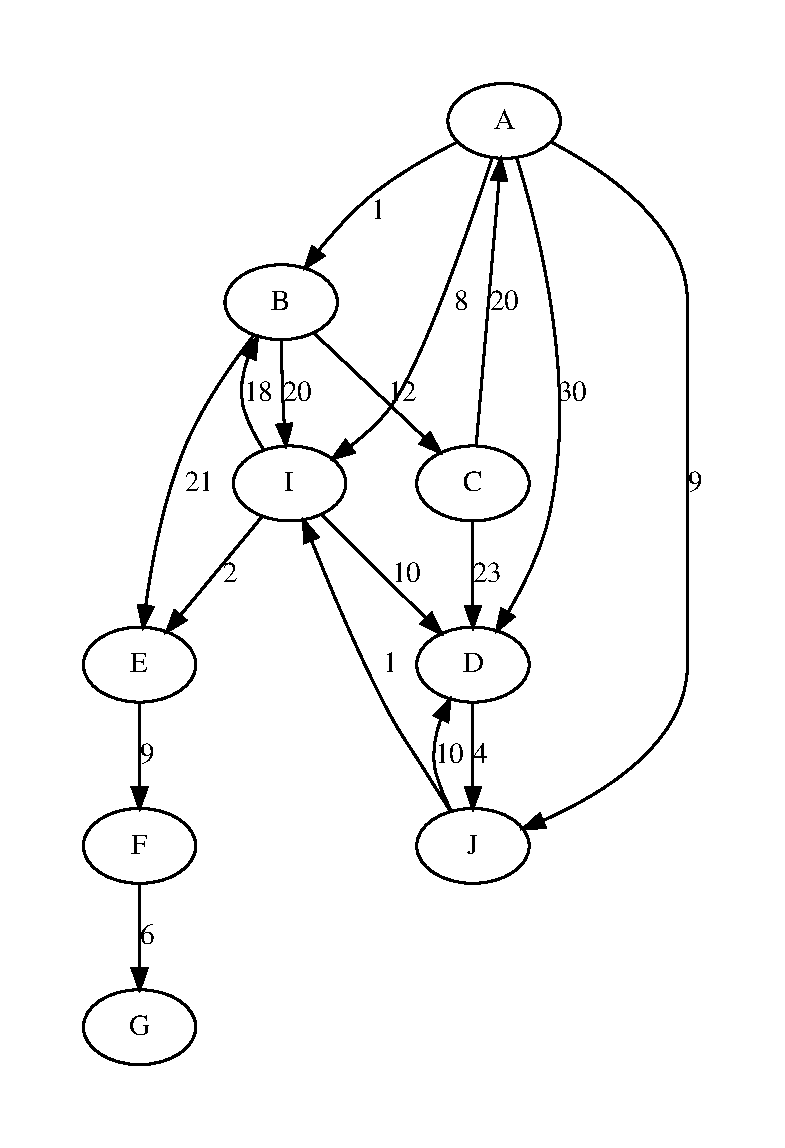
\includegraphics[width=0.5\textwidth]{../Images/Linkedg.pdf}
\end{center}
\end{itemize}
\end{column}

\end{columns}
\end{frame}

%%%%%%%%%%%%%%%%%%%%%%%%%%%%%%%%%%%%%%%%%%%%%%%%%%%%%%%%%%%%%%

\begin{frame}[fragile]
\frametitle{TSP II}
\begin{columns}[T]

\begin{column}{0.45\textwidth}
\lstinputlisting[style=basicc,linerange={5-26},numbers=none]{../../ADTs/Graph/Indep/indep.c}
\end{column}

\pause
\begin{column}{0.45\textwidth}
\lstinputlisting[style=basicc,linerange={27-46},numbers=none]{../../ADTs/Graph/Indep/indep.c}
\end{column}

\end{columns}
\end{frame}



%%%%%%%%%%%%%%%%%%%%%%%%%%%%%%%%%%%%%%%%%%%%%%%%%%%%%%%%%%%%%%

\begin{frame}[fragile]
\frametitle{Algorithms : Dijkstra on Graphs}
\begin{columns}[T]

\begin{column}{0.45\textwidth}
\begin{itemize}[<+->]
\item It's often important to find the shortest path through a graph from one vertex to another.
\item One way of doing this is the greedy algorithm due to Dijkstra discovered $~1956$.
\item Picks the unvisited vertex with the lowest distance, \& calculate the distance through it to each unvisited neighbor, updating the neighbour's distance if smaller.
\item Mark visited when done with neighbors.
\end{itemize}
\end{column}

\begin{column}{0.45\textwidth}
\begin{center}
\pause
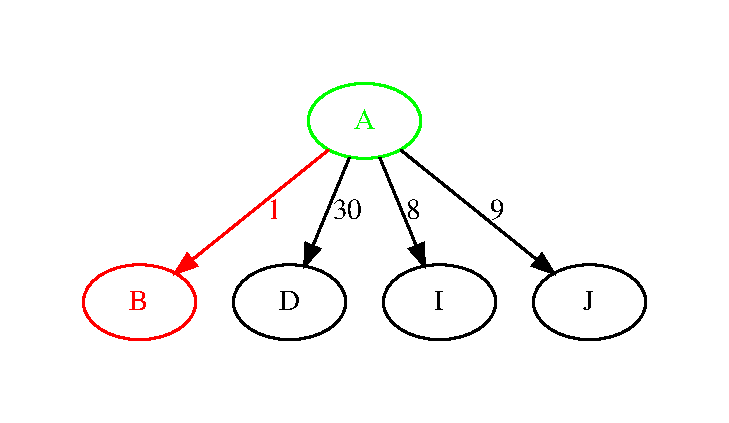
\includegraphics[width=0.4\textwidth]{../Images/dijkstra1.pdf}
\pause
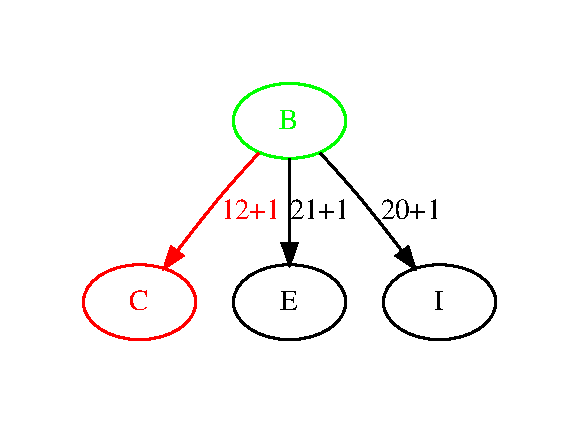
\includegraphics[width=0.4\textwidth]{../Images/dijkstra2.pdf}
\pause
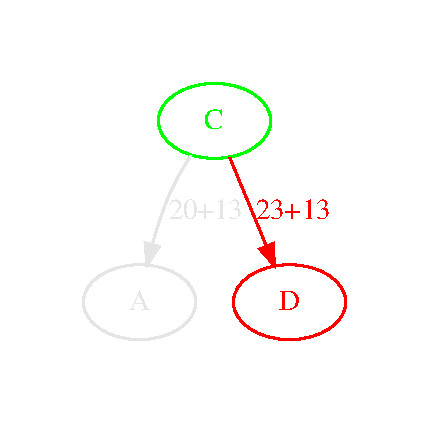
\includegraphics[width=0.4\textwidth]{../Images/dijkstra3.pdf}
\end{center}
\end{column}

\end{columns}
\end{frame}

%%%%%%%%%%%%%%%%%%%%%%%%%%%%%%%%%%%%%%%%%%%%%%%%%%%%%%%%%%%%%%
